\chapter{Abstraction Algorithm Development}
\lhead{\emph{Abstraction Algorithm Development}}
\label{chapter:abstract}

In Section \ref{Subsection:abstract} we defined data abstraction as the reduction of an image down to only its most essential elements. What these essential elements are depends on the application, leading to a large range of possible methods and results. In this implementation of data abstraction the aim is to be able to navigate a telerobot from the resultant images, therefore the most important elements of each image are the size and shape of the objects in it. It is possible to convey the rough shape of an object by presenting its outline, therefore leading to edge detection being chosen as the first step of the algorithm. Identification of objects, while possible using edges alone, is significantly easier when colour is also provided. Most of the colours in an image, however, do not aid in object identification; one colour (preferably the average colour) for each object in the scene is sufficient. This leads to the algorithm presented in Figure \ref{fig:process}, with examples of the abstractions it produces presented in Appendix \ref{Appendix:demo}.

\begin{figure}[H]
    \begin{center}
      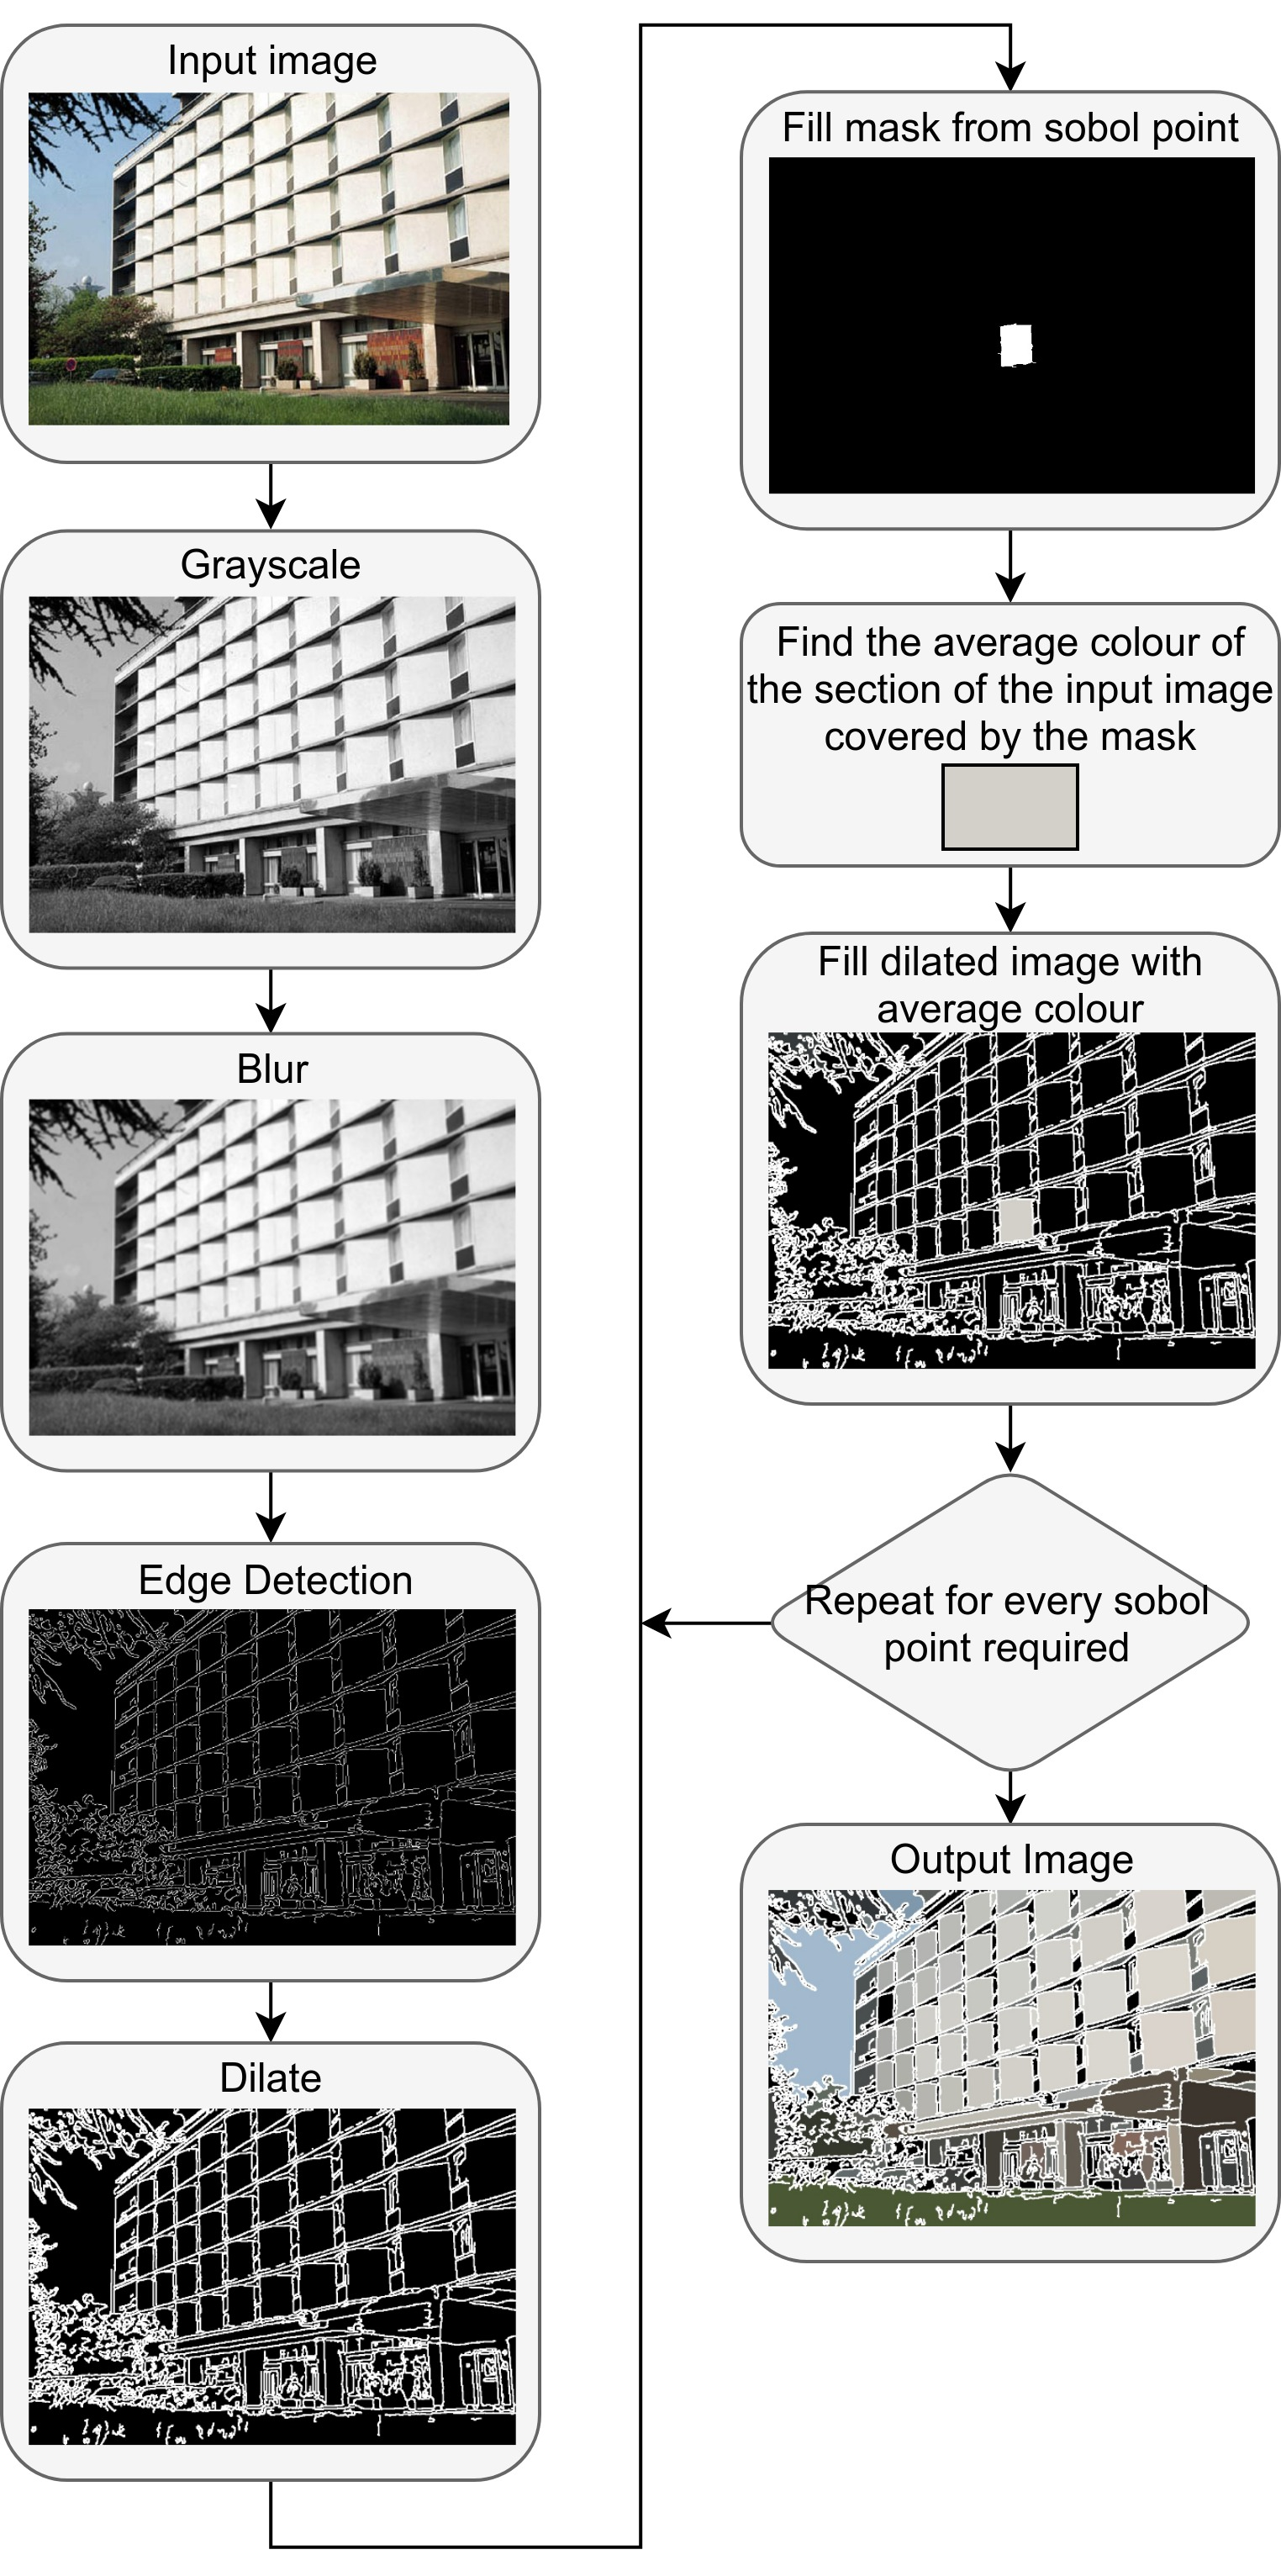
\includegraphics[width=0.75\textwidth]{Figures/Abstraction.jpg}
      \caption[Data Abstraction Algorithm Process]{Data Abstraction Algorithm Process. The left half is explained in the "Edge Detection Process" section and the right half in the "Colour Averaging" section, both located below.}
      \label{fig:process}
    \end{center}
\end{figure}

This chapter is presented in the context of the entire process occurring on a single computer; when incorporated into the final system, the whole process is undertaken on the rover apart from the "Fill dilated image with average colour" block, which is implemented on the server in its own loop through every sobol point ("Coloured Abstraction Construction" on Figure \ref{fig:system}). It is also worth noting that this chapter is concerned with the algorithm's ability to produce recognisable abstractions under reasonable resource constraints, and not the file sizes of said abstractions. The file sizes it is capable of producing will be covered as part of the system testing and evaluation in Chapter \ref{chapter:eval}.

\section{Edge Detection Process}

Canny edge detection was implemented using the Canny function provided by OpenCV \cite{OpenCV}. The image is first converted into a grayscale format, as the edge detector detects large changes in intensity and not colour. The image is then blurred to remove any unnecessary edges and noise that may be picked up. The edge detection is applied, producing white lines representing the edges on a black background. The output of the edge detection is finally dilated to make the lines thicker and bridge the gaps between the lines that are very close together. This is done to reduce the number of lines produced by areas that are dense with detail such as hair and foliage and to bridge the gaps between lines that are close together, increasing the likelihood of defined shapes being created that can be easily flood filled later.

\section{Colour Averaging}

Flood filling was chosen as the method for applying colour to the edge detected image, as it is an effective method for filling spaces of unknown size and shape that are defined by high contrast boundaries. The OpenCV flood fill function requires a seed point to start flooding from, a colour to fill with, and parameters for the filling itself (unchanged from the defaults provided by the OpenCV documentation \cite{opencvffilldemo}).

\subsection{Seed Points}

Finding the points to flood fill from is a challenge, as each image will have a different number of spaces to be filled and the spaces can be of any size and shape. Three different methods were attempted to solve this problem. The first was an attempt to use OpenCV's contour functionality to turn the lines into a set of contours and use the centre of mass of each contour (an approximation of the centre of each space) as the seed point. Unfortunately, this was unusable due to high resource requirements. The method is detailed in Appendix \ref{appendix:contour}.

Although it would by ideal to aim to flood fill from the centre of each space, it is only necessary if the intention is to be selective about which pixels are being used as seed points. It is possible to instead iterate through the whole image and flood fill from every pixel found that is not part of an edge or an already filled space. This method is effective at filling every space, and is also less resource intensive than the previous method. However, if presented with a complicated environment with many spaces to flood fill it must fill every single one, leading to unacceptable drops in frame rate.

A simple solution to the performance issues caused by complex images would be to set a maximum number of times flood fill can be used per image. However, if this is done then the seed points can no longer be selected by iterating through the whole image, as the presence of many small spaces at the top of an image would lead to larger, more important spaces not being filled at the bottom. The chosen solution to this issue is to select a set number of points quasi-randomly across the image using Sobol sequencing (explained in Section \ref{Subsection:sobol}). Although a certain number of points will land on lines and therefore not be used, if enough points are used then all the important spaces are filled without performance being heavily influenced by the complexity of the image as in the brute force method above (Figure \ref{fig:fpscomp}). However, complicated images will be processed with many of their denser areas unfilled (Figure \ref{fig:BrutevsSobol}). It was decided that this was an adequate tradeoff for the performance improvements using sobol points provides, therefore the seed points are selected using this method in the final design.

\begin{figure}[H]
    \begin{center}
      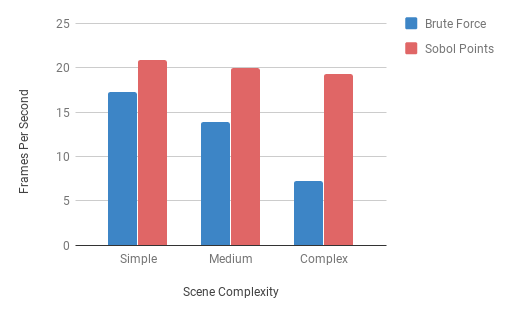
\includegraphics[width=0.9\textwidth]{Figures/FPSComp.png}
      \caption[Performance Comparison of Seed Point Methods]{Performance Comparison of Seed Point Methods. It can be clearly seen that as the complexity of the scene increases, the brute force method results in unacceptable drops in frame rate, whereas the sobol method maintains a much higher degree of consistency. Images of the scenes used in this test can be found in Appendix \ref{Appendix:scenes}.}
      \label{fig:fpscomp}
    \end{center}
\end{figure}

\begin{figure}[H]
    \begin{center}
    \begin{tabular}{ c c }
        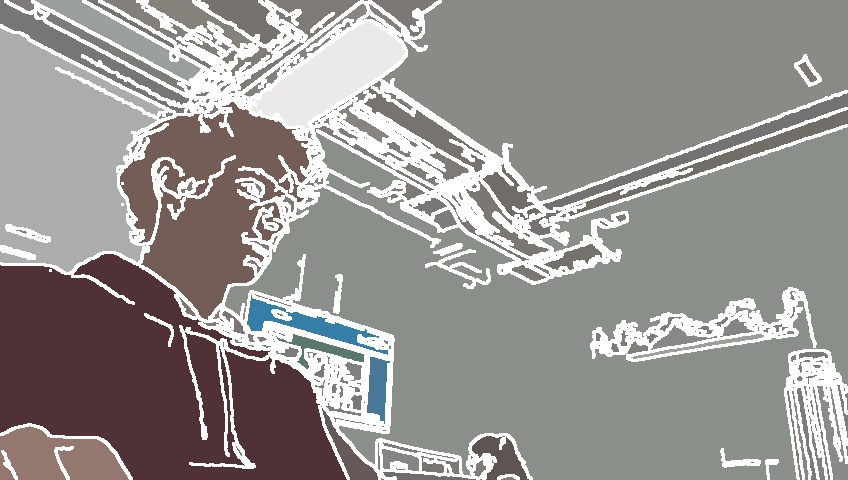
\includegraphics[width=0.45\textwidth]{Figures/Brute.jpg} &
        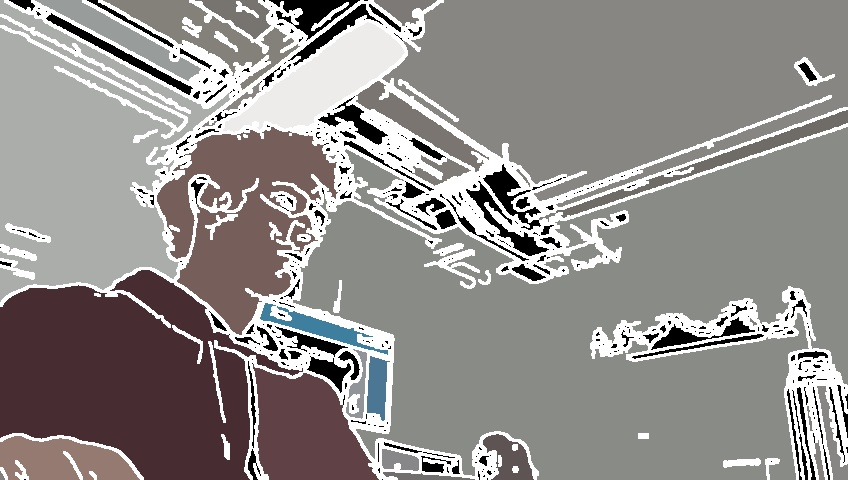
\includegraphics[width=0.45\textwidth]{Figures/Sobol.jpg}
    \end{tabular}
    \caption[Comparison of brute force and Sobol seed point generation]{Comparison of brute force and Sobol seed point generation. It can be observed that the brute force method (left) accurately fills every space in the image, whereas using the Sobol method results in many unfilled spaces.}
    \label{fig:BrutevsSobol}
    \end{center}
\end{figure}

\subsection{Fill Colour}

Three different methods were considered for finding the colours that the edge detected image must be flood filled with. All three methods are valid solutions, but present different ratios between accuracy and resource requirements.

Filling the abstracted image with the average colours of the objects present within the input image would be the clear optimal choice for the purposes of object recognition. However, the use of average colours is not essential; the objects in the scene are can still be recognisable with significantly lower colour accuracy. For this reason it would be acceptable to not find the average colour of the area being flood filled at all, and instead simply use the colour present in the input image at the seed point. This is a very fast method, however produces wildly inconsistent colours between images. This is because there can be a wide spectrum of colour across a single surface even within the threshold of Canny edge detection, and the Sobol sequence will not always sample from the same point in each new frame, producing spaces that flicker between a wide range of colours.

The consistency of the previous method can be improved substantially with minimal impact on performance by taking an average of the colour within the area of a small circle around the seed point, rather than just the colour of that one point. This significantly improves the consistency between images, however introduces the problem of incorporating pixels from outside the space in question. This is due to the quasi-random points often being so close to the edge of the space that the averaging circle crosses the edge slightly and incorporates part of a neighbouring space in the average. Therefore, the size of the circle must be carefully selected to balance the benefits of increasing size (more consistency when the seed point is near the centre of the space) and the benefits of decreasing size (more consistency when the seed point is closer to the edge). 

The OpenCV flood fill function provides the ability to fill a blank mask using the boundaries defined by a different image \cite{bradski2008learning}. This makes it possible to create a custom mask with the exact size and shape of the space that is to be filled and use that to find the average colour instead of a predefined circle. This produces the average colour of every space in the image exactly at the expense of adding an extra stage of flood filling before the edge detected image itself is filled (a stage of flood filling that has to be undertaken on the rover in the full system). The consistency between images for this is the maximum possible based on colour alone (Figure \ref{fig:ColourConsistency}), though inconsistency in the edge detection causes certain spaces to combine and divide constantly, leading to a small amount of colour inconsistency to remain regardless. The fact that this method leads to flood filling being undertaken on the rover as well as the server leads to performance concerns, however the consistency it produces led it to be the chosen method to be implemented into the full system.

\begin{figure}[H]
    \begin{center}
      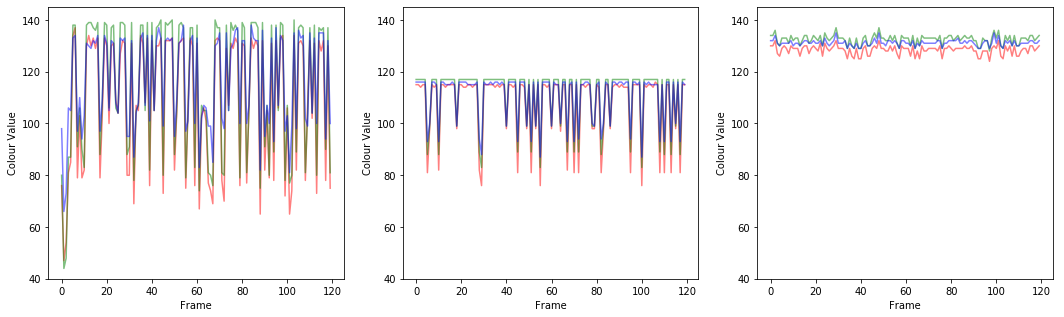
\includegraphics[width=1\textwidth]{Figures/ColourConsistency.png}
      \caption[Comparison of Colour Averaging Methods]{Comparison of Colour Averaging Methods. These are RGB values over time produced by flood filling an example area using the colour of the seed point (left), circle average (middle), and flood fill average (right). The increase in consistency from left to right is very apparent.}
      \label{fig:ColourConsistency}
    \end{center}
\end{figure}